\documentclass[aspectratio=169]{beamer}
\usepackage{beamerthemesplit}
\usepackage{wrapfig}
\usetheme{SPbGU}
\usepackage{pdfpages}
\usepackage{amsmath}
\usepackage{cmap} 
\usepackage[T2A]{fontenc} 
\usepackage[utf8]{inputenc}
\usepackage[english,russian]{babel}
\usepackage{indentfirst}
\usepackage{amsmath}
\usepackage{tikz}
\usepackage{multirow}
\usepackage[noend]{algpseudocode}
\usepackage{algorithm}
\usepackage{algorithmicx}
\usetikzlibrary{shapes,arrows}
\usepackage{fancyvrb}
\usepackage{appendixnumberbeamer}
\usepackage{xcolor,colortbl}
\usepackage{listings}
\usepackage{multicol}
\usepackage{tabularx}

\newtheorem{rutheorem}{Теорема}
\newtheorem{ruproof}{Доказательство}
\newtheorem{rudefinition}{Определение}
\newtheorem{rulemma}{Лемма}

\definecolor{mygreen}{rgb}{0,0.6,0}
\definecolor{mygray}{rgb}{0.5,0.5,0.5}
\definecolor{mymauve}{rgb}{0.58,0,0.82}

\lstset{ %
  backgroundcolor=\color{white},   % choose the background color
  basicstyle=\footnotesize,        % size of fonts used for the code
  breaklines=true,                 % automatic line breaking only at whitespace
  captionpos=b,                    % sets the caption-position to bottom
  commentstyle=\color{mygreen},    % comment style
  escapeinside={\%*}{*)},          % if you want to add LaTeX within your code
  keywordstyle=\color{blue},       % keyword style
  stringstyle=\color{mymauve},     % string literal style
  captionpos=b,
  frame=single,
  literate={->}{{$\to$}}3 {===}{{$\equiv$}}1 {=/=}{{$\not\equiv$}}1 {|>}{{$\triangleright$}}3 {\\/}{{$\vee$}}2 {/\\}{{$\wedge$}}2 {>=}{{$\ge$}}1 {<=}{{$\le$}} 1,
morecomment=[s]{(*}{*)}
}

\lstdefinelanguage{ocaml}{
keywords={@type, function, fun, let, in, match, with, when, class, type,
nonrec, object, method, of, rec, repeat, until, while, not, do, done, as, val, inherit, and,
new, module, sig, deriving, datatype, struct, if, then, else, open, private, virtual, include, success, failure,
lazy, assert, true, false, end},
sensitive=true,
commentstyle=\small\itshape\ttfamily,
keywordstyle=\ttfamily\bfseries, %\underbar,
identifierstyle=\ttfamily,
basewidth={0.5em,0.5em},
columns=fixed,
fontadjust=true,
literate={->}{{$\to$}}3 {===}{{$\equiv$}}1 {=/=}{{$\not\equiv$}}1 {|>}{{$\triangleright$}}3 {\\/}{{$\vee$}}2 {/\\}{{$\wedge$}}2 {>=}{{$\ge$}}1 {<=}{{$\le$}} 1,
morecomment=[s]{(*}{*)}
}

\beamertemplatenavigationsymbolsempty

\title[GraphBLAS F\#]{Brahma.FSharp как основа для обобщённой
разреженной линейной алгебры на GPGPU}
\institute[СПбГУ]{}
\author[Панфилёнок Дмитрий]{Панфилёнок Дмитрий Викторович}
 
\begin{document}
{
\setbeamertemplate{footline}{}
\begin{frame}
  
\includegraphics[width=1.4cm]{pictures/SPbGU_Logo.png}
\vspace{-35pt}
\hspace{-10pt}
\begin{center}
  \begin{tabular}{c}
    \scriptsize{Санкт-Петербургский государственный университет} \\
    \scriptsize{Кафедра системного программирования}
    \end{tabular}
\titlepage
\end{center}

\btVFill

{\scriptsize{\bfseries Научный руководитель:} к.ф.-м.н., доцент кафедры информатики С.~В.~Григорьев \\ }
{\scriptsize{\bfseries Рецензент:} инженер-программист ООО <<ИнтеллиДжей Лабс>> А.~В.~Бережных \\ }

\begin{center}
  \vspace{5pt}
  \scriptsize{Санкт-Петербург\\
                 2022}
  \end{center}
\end{frame}
}

\begin{frame}[fragile]  
  \frametitle{Введение}
  \begin{itemize}
    \item Использование GPGPU может повысить производительность алгоритмов анализа графов
    \item Современные инструменты достигают этого ценой более сложной модели программирования
\end{itemize}

~\\
\textbf{Стандарт GraphBLAS:}
\begin{itemize}
  	\item Графы могут быть представлены разреженными матрицами
  	\item Алгоритмы на графах можно выразить в терминах линейной алгебры над различными полукольцами
    \item Спецификация GraphBLAS описывает структуру объектов и методов для реализации таких алгоритмов в терминах линейной алгебры
  \end{itemize}
\end{frame}
     
\begin{frame}  
  \frametitle{Существующие решения}
  \begin{table}[htbp]
    \begin{tabularx}{\textwidth}{X|X|l}
      Реализация & Язык & Поддержка GPU \\
      \hline
      SuiteSparse & C & Нет \\
      GBTL & C++ & Нет \\
      GraphBLAST & C++ & CUDA \\
      CombBLAS & C++ & Частичная, CUDA \\
      Graphulo & Java & Нет \\ 
      \hline
    \end{tabularx}
  \end{table}
  
  \bigskip
  \textbf{Недостатки существующих решений:}
  \begin{itemize}
    \item Отсутствие инструментов, полностью реализующих GraphBLAS на GPU
  	\item Низкая переносимость решений, основанных на CUDA
    \item Нет самостоятельных библиотек для высокоуровневых языков
  \end{itemize}
\end{frame}

\begin{frame}  
  \frametitle{Возможное решение}
  \begin{onehalfspace}
    \textbf{Инструмент:} GraphBLAS-sharp \\
    \textbf{Поддержка GPU:} OpenCL \\
  \end{onehalfspace}
    \textbf{Язык:} F\# \\
    \begin{itemize}
      \item Проверки времени компиляции
      \item Платформа и экосистема .NET
      \item Поддержка алгебраических типов данных 
      \item Широкие возможности для метапрограммирования
    \end{itemize}
    \textbf{Использует:} Brahma.FSharp
\end{frame}

\begin{frame}  
  \frametitle{Существующие проблемы}
  \begin{enumerate}
    \item Отсутствие поддержки произвольных атомарных операций
  	\item Отсутствие поддержки трансфера пользовательских типов данных из управляемой памяти в видеопамять
    \item Неэффективное управление памятью устройства
    \item Отсутствие возможности исполнения нескольких OpenCL ядер параллельно
  \end{enumerate}
\end{frame}

\begin{frame}
  \frametitle{Постановка задачи}
    Предметом данной работы является улучшение библиотеки
Brahma.FSharp c целью её применения в инструментах для обобщённой
разреженной линейной алгебры на GPGPU.

  ~\\
  \textbf{Задачи:}
  \begin{itemize}
    \item Реализовать поддержку обобщенных атомарных операций
    \item Реализовать поддержку трансфера пользовательских типов данных
    \item Обеспечить возможность управления выделением памяти на OpenCL устройстве
    \item Обеспечить возможность параллельного исполнения OpenCL ядер
    \item Сравнить производительность полученного решения с аналогами
  \end{itemize}
\end{frame}

\begin{frame}
    \frametitle{Brahma.FSharp}
    
\textbf{Особенности:}
    \begin{itemize}
        \item Позволяет использовать подмножество языка F\# для написания ядер OpenCL
        \item Позволяет проверять некоторые ошибки на этапе компиляции
        \item Обеспечивает переносимость за счет кодогенерации
    \end{itemize}
    
\bigskip
    
    \textbf{Содержит:}
    \begin{itemize}
        \item Транслятор из F\# в OpenCL
        \item API хоста для запуска ядер и управления памятью
    \end{itemize}
    
        \begin{figure}[h!]
\centering
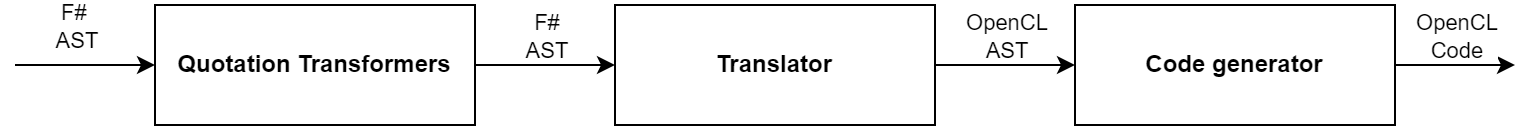
\includegraphics[scale=0.25]{pictures/Transl.drawio (2).png}
\caption{Устройство транслятора}
\end{figure}
\end{frame}

\begin{frame}[fragile]
  \frametitle{Поддержка произвольных атомарных операций}
  \begin{itemize}
      \item Стандартные операции $\xrightarrow{}$ вызов встроенных атомарных функций OpenCL
      \item Пользовательские операции $\xrightarrow{}$ вызов сгенерированных функций, реализующих спинлок
  \end{itemize}
\bigskip
\begin{lstlisting}[caption=Сигнатура функции atomic, language=Caml, frame=single, label={lst:atomic}, morekeywords={val}]
val atomic : ('a -> 'b) -> ('a -> 'b)
\end{lstlisting}
\end{frame}
            
\begin{frame}[fragile]
  \frametitle{Поддержка трансфера пользовательских типов данных}
  Методы класса \textbf{CustomMarshaler}:
\begin{itemize}
\item \verb|IsBlittable(Type): bool| --- определяет, является ли тип данных непреобразуемым
\item \verb|WriteToUnmanaged('a[]): int| --- копирует данные из управляемой памяти в неуправляемую
\item \verb|ReadFromUnmanaged(IntPtr, length: int): unit| --- копирует данные из неуправляемой памяти в управляемую
\end{itemize}

\bigskip

  \begin{minipage}{0.3\textwidth}
  \textbf{Было:}
  \begin{itemize}
    \item int
    \item double
    \item sbyte
    \item \ldots
  \end{itemize}
\end{minipage}
\hfill
\begin{minipage}{0.55\textwidth}
  \textbf{Добавлено:}
  \begin{itemize}
    \item Структуры
  	\item Кортежи
    \item Записи
    \item Размеченные объединения
  \end{itemize}
\end{minipage}
\\
\end{frame}
       
\begin{frame}  
  \frametitle{Существующие проблемы, связанные с управлением памятью}
    \begin{itemize}
    \item Невозможно выделять память напрямую на OpenCL устройстве
    \item Невозможно выставлять нужные флаги буфера при создании
    \item Невозможно автоматически освобождать выделенную память
\end{itemize}
\end{frame}
             
\begin{frame}
    \frametitle{Управление памятью}
    \begin{figure}
\centering
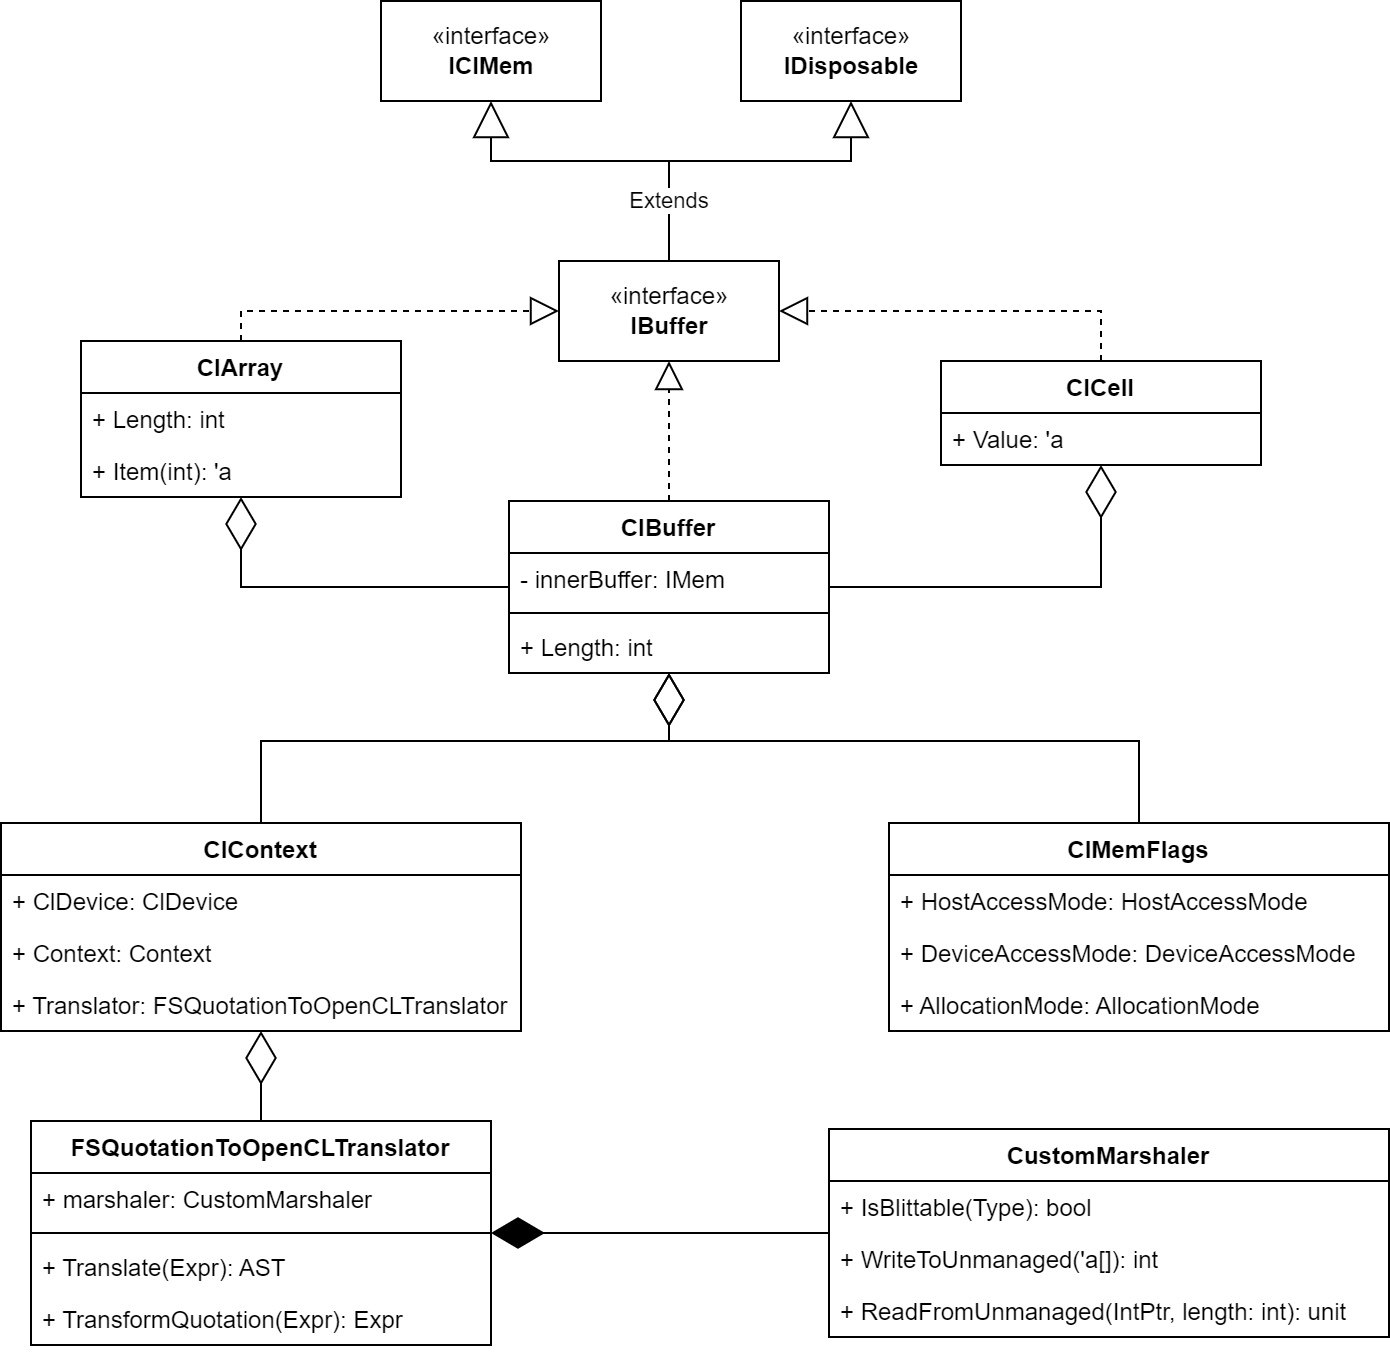
\includegraphics[scale=0.13]{pictures/Mem.drawio (1).png}
\caption{Иерархия абстракций для управления памятью}
\label{fig:mem}
\end{figure}
\end{frame}
           
\begin{frame}
    \frametitle{Архитектура решения}
    \begin{figure}
\centering
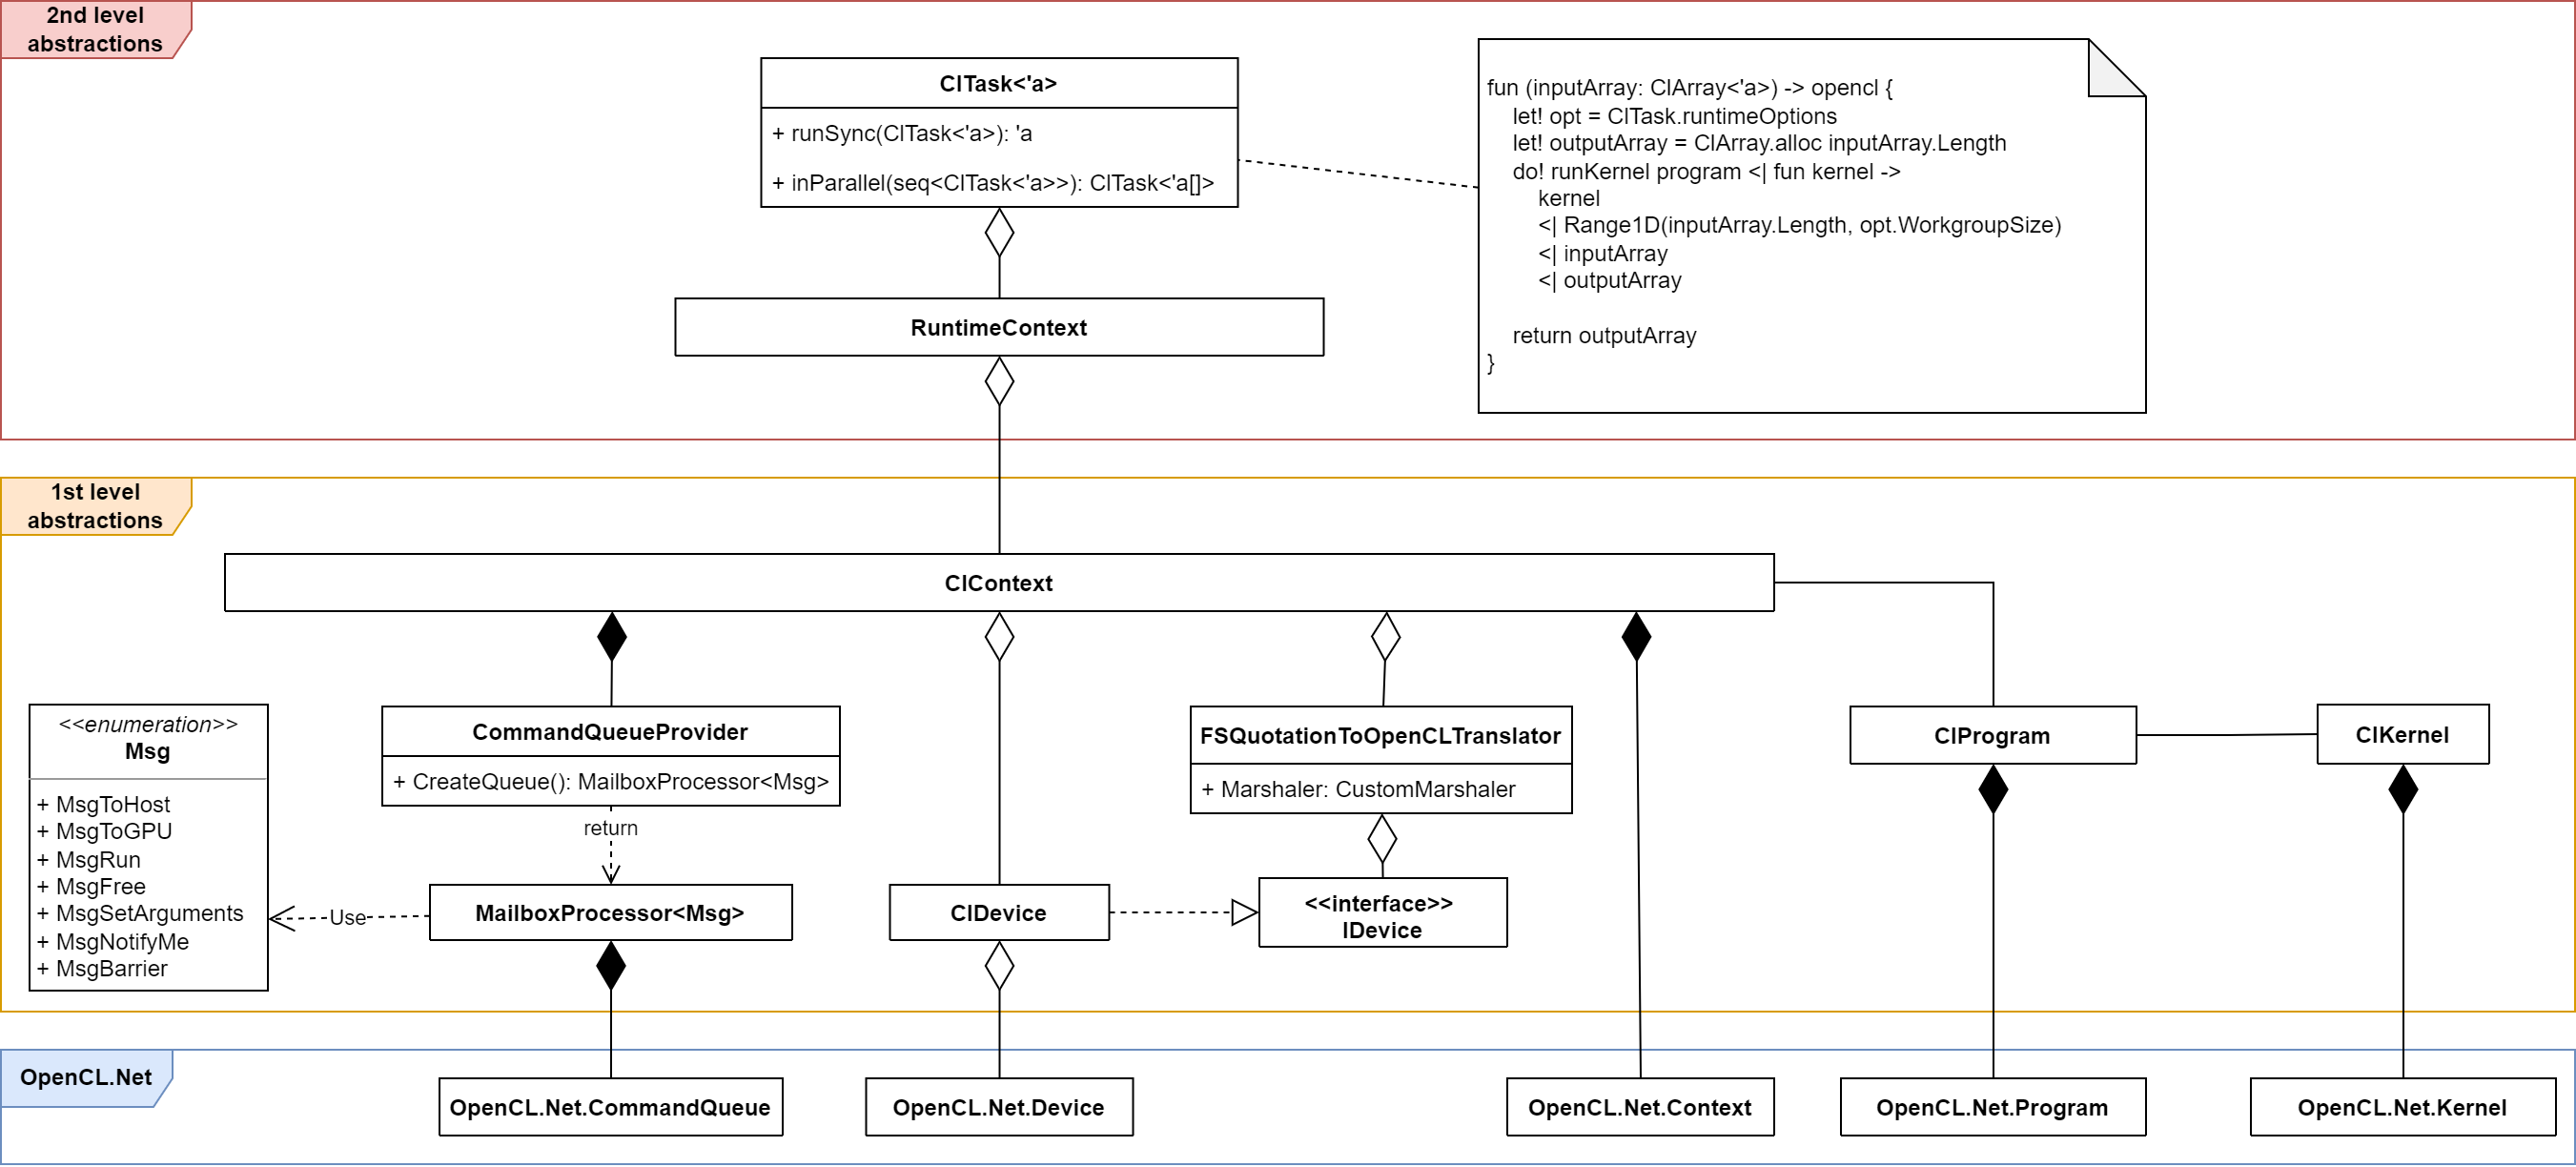
\includegraphics[scale=0.14]{pictures/small.drawio (2).png}
\caption{Архитектура решения}
\label{fig:mem}
\end{figure}
\end{frame}
           
\begin{frame}
\frametitle{Сравнение с аналогами}
\begin{table}[h]
    \begin{tabularx}{\textwidth}{|X|c|c|c|}
      \hline
      \textbf{Характеристика} & \textbf{Brahma.FSharp} & \textbf{FSCL} & \textbf{ILGPU} \\
      \hline
      Поддержка непреобразуемых типов данных & Да & Да & Да \\
      Поддержка обобщенных структур данных & Да & \textit{Нет} & Да \\
      Поддержка преобразуемых типов данных & Да & Да & \textit{Нет} \\
      \hline
      Поддержка произвольных атомарных операций & Да & \textit{Нет} & Да \\
      Поддержка параллельного исполнения команд & Да & Да & Да \\
      \hline
    \end{tabularx}
  \caption{Сравнение с аналогами}
  \label{tab:comp}
\end{table}
\end{frame}

\begin{frame}
    \frametitle{Оценка затрат на трансфер данных: запись}
    \begin{table}
    \begin{tabularx}{\textwidth}{|X|X|X|X|}
      \hline
      \textbf{Библиотека} & \textbf{Длина массива} & \textbf{Среднее, мкс} & \textbf{Стандартная ошибка, мкс} \\
      \hline
      Brahma.FSharp & 1000 & 39 & 3  \\
      ILGPU & 1000 & 45 & 2  \\
      \hline
      Brahma.FSharp & 1\,000\,000 & 2,507  & 292  \\
      ILGPU & 1\,000\,000 & 1,082 & 94 \\
      \hline
    \end{tabularx}
  \caption{Оценка времени записи данных в видеопамять, непреобразуемый тип данных ValueOption<int>}
  \label{tab:blit-w}
\end{table}

\begin{table}
    \begin{tabularx}{\textwidth}{|X|X|X|X|}
      \hline
      \textbf{Библиотека} & \textbf{Длина массива} & \textbf{Среднее, мкс} & \textbf{Стандартная ошибка, мкс} \\
      \hline
      Brahma.FSharp & 1000 & 2,685 & 418  \\
      \hline
      Brahma.FSharp & 1\,000\,000 & 2,044,113  & 48,098 \\
      \hline
    \end{tabularx}
  \caption{Оценка времени записи данных в видеопамять, преобразуемый тип данных bool}
  \label{tab:nonblit-w}
\end{table}
\end{frame}

\begin{frame}
    \frametitle{Оценка затрат на использование атомарных операций}
   \begin{table}
    \begin{tabularx}{\textwidth}{|l|X|X|X|}
      \hline
      \textbf{Реализация} & \textbf{Размер пространства} & \textbf{Среднее, мкс} & \textbf{Стандартная ошибка, мкс} \\
      \hline
      Brahma.FSharp (нативная) & 1000 & 138 & 65  \\
      Brahma.FSharp (пользовательская) & 1000 & 96 & 26  \\
      ILGPU (нативная) & 1000 & 20 & 8   \\
      ILGPU (пользовательская) & 1000 & 631 & 88  \\
      \hline
      Brahma.FSharp (нативная) & 100\,000 & 126   & 40  \\
      Brahma.FSharp (пользовательская) & 100\,000 & 298   & 42  \\
      ILGPU (нативная) & 100\,000 & 14  & 4 \\
      ILGPU (пользовательская) & 100\,000 & 541,701   & 7,757 \\
      \hline
      Brahma.FSharp (нативная) & 10\,000\,000 & 366 & 45    \\
      Brahma.FSharp (пользовательская) & 10\,000\,000 & 14,484  & 4,588    \\
      \hline
    \end{tabularx}
  \caption{Оценка затрат на использование атомарных операций}
  \label{tab:atom}
\end{table}
\end{frame}
             
\begin{frame}  
  \frametitle{Результаты}
  \begin{itemize}
\item Реализована поддержка обобщенных атомарных операций
\item Реализована поддержка трансфера обобщенных типов данных, таких как структуры, кортежи и размеченные объединения
\item Улучшена модель управления памятью
\item Переработана архитектура библиотеки
\item Реализована возможность параллельного исполнения ядер OpenCL
\item Проведено экспериментальное сравнение предложенной реализации с аналогами
\end{itemize}
\end{frame}         

\end{document}